% !TeX program = lualatex
\documentclass[12pt, a5paper]{article}
\usepackage{fullpage}
\usepackage{subfiles}
\usepackage{fontspec}
\usepackage{libertine}
\usepackage{xcolor}
\usepackage{GotIn}
\usepackage{geometry}
\usepackage{multicol}
\usepackage{multicolrule}
\usepackage{graphicx}
\usepackage{enumitem}
\usepackage[autocompile]{gregoriotex}

\geometry{top=1cm, bottom=1cm, right=1cm, left=1cm}
\pagestyle{empty}

\definecolor{red}{HTML}{C70039}
% \input GoudyIn.fd
% \newcommand*\initfamily{\usefont{U}{GoudyIn}{xl}{n}}

\input Acorn.fd
\newcommand*\initfamily{\usefont{U}{Acorn}{xl}{n}}
% cette ligne ajoute de l'espace entre les portées
% \grechangedim{baselineskip}{60pt}{scalable}

\begin{document}
\gresetlinecolor{gregoriocolor}
\small

\begin{titlepage}\centering
  \vspace*{\fill}\
  \huge Secondes Vêpres\\
  \large des dimanches ordinaires\\
  \smallskip
  \begin{footnotesize}
    \textit{
      Les dimanches de Carême.\\
    }
  \end{footnotesize}
  \medskip
  \large et\\
  \medskip
  \LARGE Salut du Saint-Sacrement
  \bigskip
  \begin{figure}[h!]
    \centering
    
\includegraphics[width=7cm]{logo.png}
  \end{figure}

  \vspace*{\fill}
  \large\textit{
    Livret latin-français
  }
\end{titlepage}

\begin{center}
  \rule{2cm}{0.4pt}
\end{center}

\vspace{5mm}
\begin{center}
  \textcolor{red}{\normalsize{Ouverture.}}
\end{center}

% greillumination: remplace la première lettre, ici par une font ornementale
\greillumination{\initfamily\fontsize{11mm}{11mm}\selectfont D}
\gregorioscore{vepres-deus_in_adjutorium}
\medskip

\begin{center}
  \small{
  \emph{
    Dieu, venez à mon aide ; Seigneur, hatez-vous de me secourir.\\
    Gloire au Père, au Fils et au Saint Esprit, comme il était au commencement, maintenant et toujour et dans les siècles des siècles.\\
    Ainsi soit-il. Alleluia.
  }
}
\end{center}


% \gregorioscore{vepres-deus_in_adjutorium_septuagesime}

% vfill : prends l'espace vertical disponible 
% \vfill

\begin{center}
  \rule{2cm}{0.4pt}
\end{center}
% greseparator: ornement. Le premier parametre est le type (de 1 à 5), le second la taille en points
% \greseparator{4}{30}

\newpage

\subfile{psaumes-dimanches-ordinaires.tex}

% \newpage

% \begin{center}
%   \rule{2cm}{0.4pt}
% \end{center}

% \vspace{5mm}
\begin{center}
  \textcolor{red}{\normalsize{Capitule.}}\\
  \footnotesize{
    \emph{Au propre du jour}
  }
\end{center}


% \begin{center}
%   \rule{2cm}{0.4pt}
% \end{center}

% \newpage

\begin{center}
  \rule{2cm}{0.4pt}
\end{center}

\begin{center}
  \textcolor{red}{\normalsize{Hymne.}}\\
  \begin{footnotesize}
    \textit{
      Sauf Dimanche de la Passion et Dimanche des Rameaux, \\
      voir au propre du jour.
    }
  \end{footnotesize}
\end{center}

% \grechangedim{baselineskip}{70pt}{scalable}

\gresetinitiallines{1}
\greillumination{\initfamily\fontsize{11mm}{11mm}\selectfont A}
\gregorioscore{hymnes/hy--audi_benigne_conditor--solesmes}
\bigskip

\begin{footnotesize}
  \parindent=0pt
  \begin{enumerate}[label=\textcolor{red}{\emph{\arabic*}}]
    \item \textit{Créateur plein de bonté, écoutez les
    prières, et regardez les larmes dont
    nous accompagnons le jeûne sacré de
    cette sainte quarantaine.}
    \item \textit{Il est vrai que nous avons beaucoup
    péché; mais pardonnez-nous, en
    considération de l'humble aveu que nous
    vous en faisons; et pour la gloire de
    votre nom, guérissez nos âmes malades.}
    \item \textit{Père des miséricordes, scrutateur des
    cœurs, vous connaissez notre faiblesse;
    pardonnez à des enfants qui reviennent
    sincèrement à vous.}
    \item \textit{Faites que, pendant que nos corps seront
    mortifiés par l'abstinence, nos âmes par
    un jeûne plus saint, s'abstiennent de tout
    péché.}
    \item \textit{O bienheureuse Trinité,
    qui êtes un seul Dieu,
    que votre grâce rende utile à vos serviteurs
    l'offrande qu'ils vous font de leurs jeûnes. Amen.}
  \end{enumerate}
\end{footnotesize}
% \grechangedim{baselineskip}{50pt}{scalable}

\begin{center}
  \rule{2cm}{0.4pt}
\end{center}

\newpage


\gresetinitiallines{0}
\gabcsnippet{(c3)<c><v>\Vbar</v>.</c> An(h)ge(h)lis(h) sù(h)is(h) Dé(h)us(h) man(h)dá(h)vit(h) de(h) te.(g'_) (hvGF'Efgf.) (::) (Z) <c><v>\Rbar</v>.</c> Ut(h) cu(h)stó(h)di(h)ant(h) te(h) in(h) óm(h)ni(h)bus(h) vi(h)is(h) tu(h)is.(g'_) (hvGF'Efgf.) (::)}
\smallskip
\begin{center}
  \textit{\textcolor{red}{\Vbar.} Dieu a commandé à ses Anges,\\
  \textcolor{red}{\Rbar.} De vous garder dans toutes vos voies.}
\end{center}

\begin{center}
  \rule{2cm}{0.4pt}
\end{center}

\begin{center}
  \textcolor{red}{\normalsize{Cantique de la Bienheureuse Vierge Marie}}\\
  \footnotesize{
    \emph{Au propre du jour}
  }
\end{center}

\begin{center}
  \rule{2cm}{0.4pt}
\end{center}

\begin{center}
  \textcolor{red}{\normalsize{Oraison}}\\
  \footnotesize{
    \emph{Au propre du jour}
  }
\end{center}

\begin{center}
  \rule{2cm}{0.4pt}
\end{center}

\begin{center}
  \textcolor{red}{\normalsize{Conclusion de l'office}}
\end{center}


\begin{multicols}{2}
  \parindent=0pt
  \begin{flushright}
    \textcolor{red}{\Vbar.} Dominus vobiscum.\\
    \textcolor{red}{\Rbar.} Et cum spiritu tuo.\\
  \end{flushright}

  \columnbreak
  
  \textit{\textcolor{red}{\Vbar.} Le Seigneur soit avec vous.\\
  \textcolor{red}{\Rbar.} Et avec votre esprit.}\\
\end{multicols}

\vspace{10pt}

\gresetinitiallines{1}
\greillumination{\initfamily\fontsize{11mm}{11mm}\selectfont B}
\gregorioscore{benedicamus/or--benedicamus_domino_(sundays_of_advent_and_lent)--solesmes_1961}

\newpage

\begin{center}
  \textcolor{red}{\normalsize{Salut du Très Saint Sacrement}}\\
  \textit{Chant d'exposition}
\end{center}

\smallskip
\begin{figure}[h!]
  \centering
  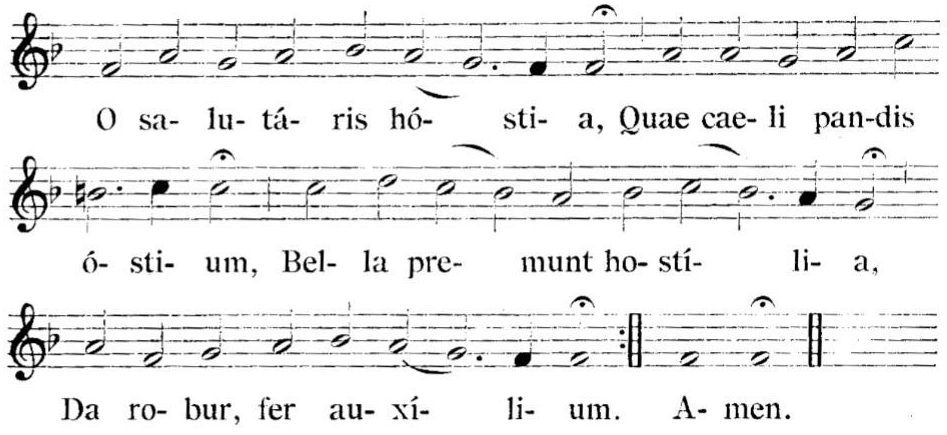
\includegraphics[width=\linewidth]{o-salutaris.jpg}
\end{figure}

\begin{center}
  \begin{footnotesize}
    \textit{
      Ô réconfortante
      Hostie, Qui nous
      ouvres les portes du
      ciel, les armées ennemies
      nous poursuivent,
      Donne-nous la force,
      porte-nous secours.
    }
  \end{footnotesize}
\end{center}

\begin{multicols}{2}
  \parindent=0pt
  \begin{flushright}
    O vere digna Hostia,\\
    Spes unica fidelium,\\
    In te confidit Francia,\\
    Da pacem, serva lilium.\\
  \end{flushright}
  \columnbreak
  \textit{
    Ô vraiment digne Hostie,\\
    Unique espoir des fidèles,\\
    en toi se confie la France,\\
    Donne-lui la paix, conserve le lys.\\
  }
\end{multicols}
\begin{multicols}{2}
  \begin{flushright}
    Uni trinoque Domino\\
    Sit sempiterna gloria :\\
    Qui vitam sine termino,\\
    Nobis donet in patria. Amen.\\
  \end{flushright}
  \columnbreak
  \textit{
    Au Seigneur unique en trois personnes,\\
    La gloire éternelle;\\
    qu'il nous donne en son Royaume\\
    La vie qui n'aura pas de fin. Amen\\
  }
\end{multicols}

\begin{center}
  \rule{2cm}{0.4pt}
\end{center}


\begin{center}
  \textcolor{red}{\normalsize{Antienne à la Sainte Vierge.}}\\
  \textit{Au propre du jour}
\end{center}

\begin{center}
  \rule{2cm}{0.4pt}
\end{center}

\begin{center}
  \textcolor{red}{\normalsize{En l'honneur Du Saint Sacrement}}
\end{center}

\gresetinitiallines{1}
\greillumination{\initfamily\fontsize{11mm}{11mm}\selectfont T}
\gregorioscore{hy--tantum_ergo--solesmes}

\begin{center}
  \begin{footnotesize}
    \begin{enumerate}[label=\textcolor{red}{\emph{\arabic*}}]
      \item \textit{Devant un sacrement si grand, prosternons-nous, adorons ; et que les symboles anciens s'effacent devant le rite nouveau ; que la foi vienne suppléer à la faiblesse de nos sens.}
      \item \textit{Au Père et au Fils louanges et acclamations, gloire honneur et puissance ainsi que bénédictions. A Celui qui de tous deux procède offrons une égale louange.}
    \end{enumerate}
  \end{footnotesize}
\end{center}

\medskip

\begin{multicols}{2}
  \parindent=0pt
  \textcolor{red}{\Vbar.} Panem de caelo praestitisti eis.\\
  \textcolor{red}{\Rbar.} Omne delectamentum in se habentem.\\
  
  \textit{\textcolor{red}{\Vbar.} Tu leur a donné le pain du ciel.\\
  \textcolor{red}{\Rbar.} Toute saveur se trouve en lui.}\\
  
\end{multicols}

\begin{center}
  \rule{2cm}{0.4pt}
\end{center}

\newpage

\begin{center}
  \textcolor{red}{\normalsize{Oraison}}
\end{center}

\begin{multicols}{2}
  \parindent=0pt
  Deus, qui nobis sub sacramento mirabili
  passionis tuæ memoriam reliquisti : \textcolor{red}{~†}
  tribue, quæsumus, ita nos Corporis et
  Sanguinis tui sacra mysteria venerari, \textcolor{red}{~*} ut
  redemptionis tuæ fructum in nobis
  jugiter sentiamus.\\
  Qui vivis et regnas
  cum Deo Patre in unitate Spiritus Sancti,
  Deus, per omnia sæcula sæculorum.
  Amen.
  \columnbreak

  \textit{
    Seigneur Jésus Christ, dans cet admirable
    sacrement tu nous a laissé le mémorial de
    ta passion ; donne-nous de vénérer d’un si
    grand amour le mystère de ton Corps et de
    ton Sang, que nous puissions recueillir
    sans cesse le fruit de ta rédemption. Toi
    qui règnes avec le Père et le Saint Esprit
    pour les siècles des siècles.
    Amen. 
  }
\end{multicols}

\begin{center}
  \rule{2cm}{0.4pt}
\end{center}


\begin{center}
  \textcolor{red}{\normalsize{Louanges divines}}
\end{center}


\begin{normalsize}
  \parindent=0pt
  Dieu soit béni.\\
  Béni soit son Saint Nom.\\
  Béni soit Jésus-Christ, vrai Dieu et vrai homme.\\
  Béni soit le Nom de Jésus.\\
  Béni soit son Sacré Cœur.\\
  Béni soit son précieux Sang.\\
  Béni soit Jésus dans le très Saint Sacrement de l’autel.\\
  Béni soit l’Esprit Saint Consolateur.\\
  Bénie soit l’auguste Mère de Dieu, la très Sainte Vierge Marie.\\
  Bénie soit sa Sainte et Immaculée Conception.\\
  Bénie soit sa glorieuse Assomption.\\
  Béni soit le nom de Marie, Vierge et Mère.\\
  Béni soit Saint Joseph, son très chaste époux.\\
  Béni soit Dieu dans ses anges et dans ses saints.\\
  Seigneur, donnez-nous des prêtres.\\
  Seigneur, donnez-nous de saints prêtres.\\
  Seigneur, donnez-nous beaucoup de saints prêtres.\\
  Seigneur, donnez-nous beaucoup de saintes vocations religieuses.\\
\end{normalsize}

\begin{center}
  \rule{2cm}{0.4pt}
\end{center}

\newpage

\begin{center}
  \textcolor{red}{\normalsize{Déposition}}\\
  \textit{Psaume 116}
\end{center}

\gresetinitiallines{1}
\greillumination{\initfamily\fontsize{11mm}{11mm}\selectfont L}
\gregorioscore{ps--laudate_dominum_omnes_gentes_(psalmus_116)--solesmes}
\bigskip
\begin{footnotesize}
  \textit{
    Louez le Seigneur, tous les
    peuples ;
    Fêtez-Le, tous les pays !
    Son Amour envers nous
    S'est montré le plus fort ;
    Eternelle est la Fidélité du
    Seigneur !
    Gloire au Père, au Fils
    Et au Saint-Esprit,
    Comme il était au
    commencement,
    Maintenant et toujours,
    Pour les siècles des siècles,
    amen.
  }
\end{footnotesize}

\begin{center}
  \rule{2cm}{0.4pt}
\end{center}

\newpage

\begin{titlepage}\centering
  \vspace*{\fill}
  \LARGE Propre du temps.
  \vspace*{\fill}
\end{titlepage}

\newpage

\grechangedim{baselineskip}{50pt}{scalable}

\subfile{propre-careme.tex}
\newpage
\subfile{vierge-marie.tex}

\end{document}
